\documentclass{article}
\usepackage{graphicx}
\usepackage{array}
\usepackage{listings}
\usepackage{float}
\usepackage{url}
\usepackage{geometry}
\usepackage[utf8]{inputenc}
\usepackage[english]{babel}
\usepackage[document]{ragged2e}


\graphicspath{ {../assets/} }
\geometry{left=3.0cm,right=3.0cm,top=3.0cm,bottom=3.0cm}


\title{%
	Operating Systems \\
	\large Journal
	}

\author{Daniel Huber, Nick Gilgen and Moray Yesilgüller}

\begin{document}
\maketitle

\center{with supervision from Dr. Günther Palfinger and Dr. Christophe Bersier}
\vspace*{\fill}

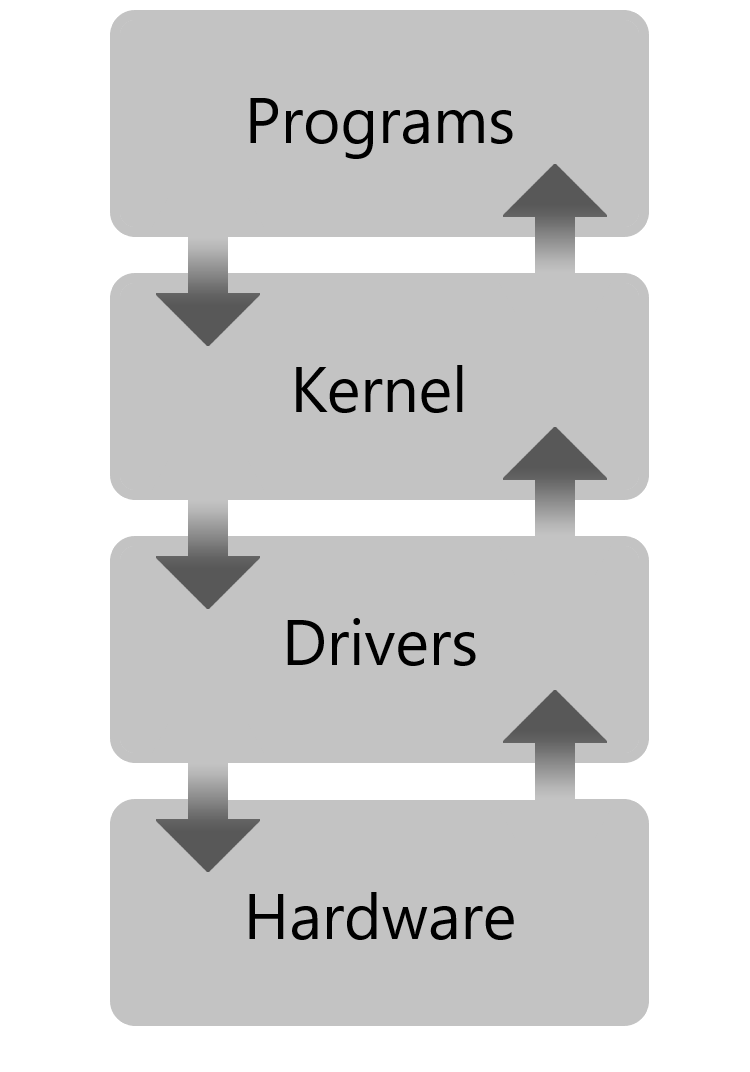
\includegraphics[width=200px]{ostp}

\bigskip
\bigskip
\bigskip
\bigskip

\center{Maturaarbeit Kantonsschule Baden}
\pagenumbering{gobble}
\newpage

\pagenumbering{arabic}
\tableofcontents


\section{Introduction}

Operating systems are essential for every working computer or mobile device. In a group of three people we tried to answer the question what operating 
systems are exactly in a booklet containing several chapters that describe the most important parts of an operating system. Additionally, we wrote our own 
operating system, including a few basic programs for entertainment.

\section{Workprocess}

\subsection{Preparation}

Our first step was deciding what our project should look like. We knew that we wanted to do something related to computer science, but we were still uncertain of the details. 
Rather spontaneously did we decide to make an operating system. The exact content of our matura project was decided after we talked to several different teachers. We 
appreciated their oppinions and we were warned of the adversities we would have to face if we chose to go through with it. The first challenge was to find find a teacher 
willing to oversee our project because we decided to write the operating system in 16-bit assembly. None of the teachers were familiar enough with assembly language, since
it is an old and nowadays rarely used programming language. Nonetheless, we embraced the challenge after we talked to Dr. Günther Palfinger. He was kind enough to accept our 
request and oversee our project. After a few weeks Dr. Palfinger reviewed the contract we set up where we decided on the terms and conditions. The second challenge was 
getting to know the assembly language. We started the research on the programing language and computer science in general even before we finished the contract. It was rather
tough in the beginning because assembly is not comparable to high-level languages like python which we picked up in school. Assembly language is much more intricate considering 
that it is closer to machine language which is the language understood by a computer. We had to invest approximately two months into research to comprehend the basics
of the language. Afterwards we each chose a task and started researching these specific topics individually. We listed the websites we used under the chapter "Sources".

\subsection{Tools}

Before we began programming we installed a virtual machine that 
allowed us to run Linux even though our host operating systems were either Windows or macOS. By using a virtual machine we protected our hardware from our own mistakes. The 
command line is a powerful tool that can, if used incorrectly, break your software and even hardware. But thanks to the virual machine we were able to isolate our host 
operating system from our working environment which was especially important as we were new to using the command line. Furthermore, Linux is commonly used by specialists 
meaning there are a lot of guides and tutorials to help beginners. On top of that, there are more and usually better, convenient, free and open-source applications. We 
then installed the Netwide Assembler or NASM for short which, as the name suggest, is an assembler. It translates the assembly source code into machine language
so that the hardware can read and execute the program. Additionally we installed QEMU, a software that allowed us to emulate an entire computer system. QEMU enabled us to 
test our programs quickly and efficiently. To write the chapters and code we used neo vim which is a text editor focused on extensibility and usability. 
It can be an extremly powerful text editor if the user is experienced. While neo vim takes some getting used to it also provides the user with convenient shortcuts. 
Sometimes our code was faulty and we needed to debug it. For convience's sake we used an online debugger called GDB. This website provided us with quick and easy access to 
a reliable debugger. In order to save time and for simplicity and consitency we also used the make utility. We created a Makefile that contains instructions for building, 
emulating and debuging software. The command make executes the Makefile in the current directory and is followed by the name of the target(s). In our project the Makefile 
launches NASM, translating the source code, and then QEMU, emulating the operating system according to the parameters defined in the Makefile. We shared the Makefiles and 
everything else we made with git. The aforementioned is a distributed version control system that allowed us to manage our project quickly and efficiently. With git one can 
upload files to and download files from a repository. We used GitHub to store our files on a cloud so that we were able to work together on this project. Finally, we used MiKTeX,
a universal document converter to convert our written text for the matura from \LaTeX \ into a pdf. All of the previously mentioned programs are free and open-source.

\subsection{Workflow}

As soon as we installed the necessary software and got a grasp of the basics of assembly language we started programming. We chose easier tasks in the beginning so that
we could warm up to this rather complicated language. Whenever we were done writing a program we began debugging it. Some bugs cost us a great amount of time which 
was often very frustrating as we lost up to three weeks because of a single bug. Fortunately, we never lost hope and always continued our research. A few times we 
had to rewrite our code because we were either stuck or unhappy with the structure. This helped a lot because we had already gained new insights by the time we started rewriting 
the program. After a while the tasks we worked on got more complicated and the research had to be more extensive. When we were not in the mood to work on the programs or do 
research we wrote chapters explaining the most important parts of an operating system. Besides that, we contributed to the work journal every week to keep Dr. Palfinger up 
to date. In the final stages of our matura project we finished writing the chapters and debugging our programs. 


\section{Product}

The main body of our project consists of a series of demo programs that work independently.
These demos can be separated into the two sections core components and gadget programs.
As the name implies, the core components play an integral part in making the operating
system work. They are as follows:


\begin{itemize}

\item \textbf{Bootloader} \\
This component is responsible for loading the kernel into memory. The kernel in FlamingOS is loosely
comprised of the remaining components listed below.
\item \textbf{Keyboard driver} \\
The keyboard driver handles the input of the keyboard through \textbf{I/O} ports. The driver 
sends a signal to a certain \textbf{I/O} port and then checks for a response containing a key
scancode. Then the response of the keyboard gets translated via a lookup table to ascii characters
or special keycodes.
\item \textbf{Shell} \\
The shell is a terminal that allows the user to send commands in the form of text via a command
line. It does this by requesting key input from the keyboard driver and saving said input
into a buffer. The command in the buffer can then be evaluated and appropriately executed.
\item \textbf{Filesystem} \\
The filesystem organizes and structures files. The filesystem is not hierarchical, meaning
that it does not support multiple directories. It provides functions for reading and writing
files and it uses a superblock to organise the files.
\item \textbf{CPU identification} \\
The CPU identification gives information on the CPU used by the computer. This is done via the 
CPUID instruction and gives information such as its manufacturer, brand, CPU family, model and
whether it is a 64 bit processor.
\item \textbf{Library} \\
The library is a collection of functions that are used across various programs. The instructions
on the usage of these functions can be found in the file \texttt{library.asm} which is located
in the \texttt{demos} directory. The library contains the following functions: 
\begin{itemize}
\item \texttt{formatHex}: Formats a numeric value to the corresponding hexadecimal ascii representation.
\item \texttt{printBuff}: Print buffer functions that prints out a buffer onto the screen. 
\item \texttt{shutdown}: Shuts down the PC. 
\item \texttt{clear\_screen}: Wipes the entire screen blank.
\item \texttt{getStringLength}: Returns the length of a string.
\end{itemize}

\item \textbf{Interrupt handlers} \\
The interrupt handler takes care of exceptions such as division by zero, double fault
and invalid opcode errors.


\end{itemize}

And of course there are also \textit{gadget programs}:

\begin{itemize}

\item Painting Program \\
In the painting program the user can draw squares with four-bit colors. It has both a cursor and an indicator 
that displays the currently selected color. There is only one brush size at the moment and the
shape of the brush is a square.

\item Hangman \\
The program hangman is a game in which the player has to guess a word that was randomly chosen from a list. The program 
reveals whether the player chose a correct character after every keyboard input. If the player guessed correctly
the game continues, but the player gets one strike if a character that is not in the randomly selected word 
was chosen. The game ends when either the player guesses all the characters in the word or three strikes have
been accumulated.

\item Texteditor \\
The texteditor program allows the user to write and delete text via keyboard input and navigate through the written 
text to correct mistakes.

\end{itemize}



There are also some other minor gadget programs not worth mentioning brcause they mostly consist of minor functions 
that were needed for specific tasks. The entire project is licenced under the GNU general public licence version 
3.0. This licence requires all modification and usage of our project to be under the same licence and 
require authors to reveal the full source code of the licenced medium. The entirety of the project is located
in a GitHub repository under the following link:

\url{https://github.com/HubDanDevMan/matura.git}

And the full licence text can be found under:

\url{https://github.com/HubDanDevMan/matura/blob/master/LICENSE}

\section{Reflection}

In hindsight, we realized that our advisors Dr. Palfinger and Dr. Bersier were right; creating 
an operating system from scratch is \textbf{hard}. In modern programming languages you have a
lot of safety nets that will save you from making mistakes and assembly has none of these nets.
Assembly is a programming language that is very close to the hardware which further distances 
the code from the actual function of the written code. There are times when we have hit
walls that simply needed time to overcome because finding the nature of a problem in assembly
is not easy. Often we had to take three steps back to take one forward, even starting anew on
a program to gain a new perspective on a problem that seemed unsolvable. Assembly programming 
can be seen as operating on a black box, you get no information on what your program does or
what's wrong with it, you simply have to look at the code long enough until you find the problem.
But as is with all programming languages over time you get better at this kind of problem solving.
But even with all the adversities that came along with OS developement we are glad that we took up
the challenge because we have gained profound insight on computers and programming. All this
newfound knowledge can be used in high-level programming languages. Despite the hardships we have 
faced, we are glad that we took up this endeavor and we will keep working on this project as we please.



\end{document}